\section{Вращательное движение твердого тела}
%Сив362
\begin{wrapfigure}[8]{R}{3cm}
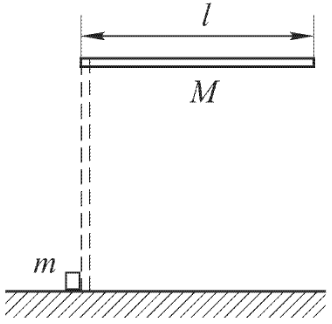
\includegraphics[width=0.25\textwidth]{rodHitMass.png}
\caption{}
\label{rodHitMass}
\end{wrapfigure}
\AddProb Стержень массы $M$ и длины $l$, который может свободно
вращаться вокруг неподвижной горизонтальной оси, проходящей через
один из его концов, под действием силы тяжести переходит из горизонтального положения в вертикальное (рис. \ref{rodHitMass}). Проходя через вертикальное положение, нижний конец стержня упруго ударяет о малое тело массы $m$, лежащее на гладком горизонтальном столе. Определить скорость тела $m$ после удара.

%Сив373
\begin{wrapfigure}[9]{R}{3cm}
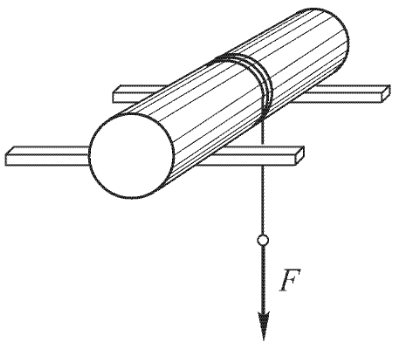
\includegraphics[width=0.25\textwidth]{rollingCylinder2.png}
\caption{}
\label{rollingCylinder2}
\end{wrapfigure}
\AddProb На двух параллельных горизонтальных брусьях лежит сплошной цилиндр радиуса $R$ и массы $m$, на который намотана веревка. К опущенному вниз концу веревки приложена вертикальная сила $F$, равная половине веса цилиндра (рис. \ref{rollingCylinder2}). Найти горизонтальное ускорение цилиндра и минимальное значение коэффициента трения между цилиндром и брусьями, при котором будет происходить качение без скольжения. Ось цилиндра перпендикулярна к брусьям, центр его масс и сила $F$ лежат в вертикальной плоскости, проходящей посередине между брусьями.

\begin{wrapfigure}[10]{R}{2.3cm}
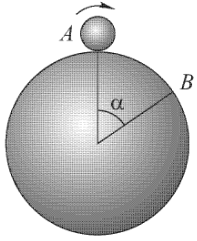
\includegraphics[width=0.2\textwidth]{ballSphere.png}
\caption{}
\label{ballSphere}
\end{wrapfigure}
%Сив383
\AddProb Шарик радиуса $r$ скатывается без начальной скорости и без скольжения по поверхности сферы из самого верхнего положения $A$ (рис. \ref{ballSphere}). Определить положение точки $B$, в которой он оторвется от сферы и начнет свободно двигаться под действием силы тяжести.
%Сив393
\AddProb Сплошной однородный шар радиуса $r$, вращающийся вокруг
горизонтального диаметра с угловой скоростью $\omega_0$, ставится на горизонтальную плоскость без сообщения ему поступательного движения. Учитывая трение скольжения, но пренебрегая трением качения, найти линейную скорость $v$ центра шара, когда его движение перейдет в чистое качение. Определить потерю кинетической энергии на трение.
%Сив366
\AddProb Вертикальный столб высотой $l$ подпиливается у основания и падает на землю, поворачиваясь вокруг нижнего основания. Определить линейную скорость его верхнего конца в момент удара о землю. Какая точка столба будет в этот момент иметь ту же скорость, какую имело бы тело, падая с той, же высоты, как и данная точка?
%Сив369
\AddProb Гимнаст на перекладине выполняет большой оборот из стойки на руках, т.е. вращается, не сгибаясь, вокруг перекладины под действием собственного веса. Оценить приближенно наибольшую нагрузку $F$ на его руки, пренебрегая трением ладоней о перекладину.

\begin{wrapfigure}[30]{r}{5cm}
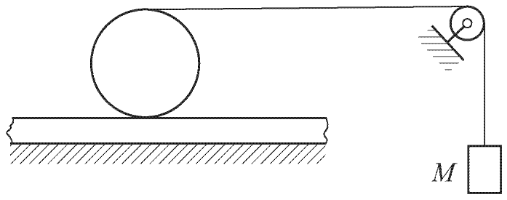
\includegraphics[width=0.4\textwidth]{slipCylinder.png}
\caption{}
\label{slipCylinder}
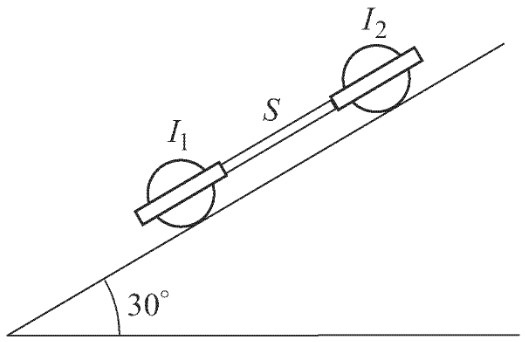
\includegraphics[width=0.4\textwidth]{2rolling.png}
\caption{}
\label{2rolling}
\centering
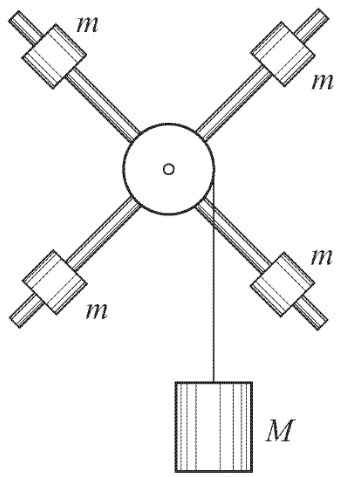
\includegraphics[width=0.3\textwidth]{oberbek.png}
\caption{}
\label{oberbek}
\end{wrapfigure}
%Сив374
\AddProb К концу веревки, намотанной на цилиндр привязан груз массы $M$. Веревка переброшена через блок, как показано на рис. \ref{slipCylinder}. Определить ускорение груза $M$. Выяснить условия, при которых качение цилиндра будет происходить со скольжением. Весом веревки и блока, а также силами трения на оси блока можно пренебречь. Считать, что во всех случаях движение цилиндра будет плоскопараллельным.
%Сив376
\AddProb Два катка, связанные штангой $S$, скатываются без скольжения с наклонной плоскости, образующей угол в $30^{\circ}$ с горизонтом (рис. \ref{2rolling}). Катки имеют одинаковые массы $m = 5$ кг и одинаковые радиусы $R = 5$ см, момент инерции первого $I_1 = 80$ кгсм\textsuperscript{2}, второго $I_2 = 40$ кгсм\textsuperscript{2}. Массами рам катков и штанги можно пренебречь. Подсчитать угловое ускорение, с которым катки скатываются без скольжения с наклонной плоскости. Определить силу, передаваемую штангой, если каток с большим моментом инерции движется впереди, и наоборот.
%Сив379.
\AddProb К шкиву креста Обербека (рис. \ref{oberbek}) прикреплена нить, к которой подвешен груз массы $M = 1$ кг. Груз опускается с высоты $h = 1$ м до нижнего положения, а затем начинает подниматься вверх. В это время происходит «рывок», т.е. увеличение натяжения нити. Найти натяжение нити $T$ при опускании или поднятии груза, а также оценить приближенно натяжение во время рывка $T_1$. Радиус шкива $r = З$ см. На кресте укреплены четыре груза с массой $m = 250$ г каждый на расстоянии $R = 30$ см от его оси. Моментом инерции самого креста и шкива пренебречь по сравнению с моментом инерции грузов. Растяжение нити во время рывка не учитывать.
%Сив391
\AddProb Сплошной цилиндр, ось которого горизонтальна, движется без вращения по гладкой горизонтальной плоскости в направлении,
перпендикулярном к его оси. В некоторый момент цилиндр достигает
границы, где поверхность становится шероховатой и возникает постоянная (не зависящая от скорости) сила трения скольжения, а трение качения отсутствует. Каково будет движение цилиндра после перехода границы? Как распределится кинетическая энергия поступательного движения цилиндра?
\clearpage